\documentclass[preview]{standalone}

\usepackage{amsmath}
\usepackage{amssymb}
\usepackage{tikz}
\usepackage{stellar}
\usepackage{definitions}

\begin{document}

\id{finite-abelian-group-element-orders}
\genpage

\section{Cyclic groups}

%\includesnpt{euler-totient-function-definition}
%\includesnpt{euler-totient-of-prime}
%\includesnpt{euler-totient-of-prime-power}
%\includesnpt{euler-totient-function-lemma1}
%
%\includesnpt{order-of-power-of-group-element-theorem}
%\includesnpt{order-of-power-of-group-element-proof}
%
%\includesnpt{cyclic-subgroups-order-classification-theorem}
%\includesnpt{cyclic-subgroups-order-classification-theorem-proof}
%
%\includesnpt{integer-sum-of-eulertotient}
%\includesnpt{integer-sum-of-eulertotient-proof}

\section{Direct products}

%\includesnpt{external-direct-product-element-period}
%\includesnpt{external-direct-product-element-period-proof}

\begin{snippetexample}{two-cyclic-groups-element-order-example}{Element orders in a product of two cyclic groups}
    Let
    \[
        G=C_n\cartesianprod C_m,
        \qquad
        C_n=\gengrp{g},
        \qquad
        C_m=\gengrp{h}.
    \]
    Every element has the form \((g^{k_1},h^{k_2})\), and
    \[
        \elementperiod{(g^{k_1},h^{k_2})}
        =
        \lcm\left(
            \elementperiod{g^{k_1}},
            \elementperiod{h^{k_2}}
        \right).
    \]
\end{snippetexample}

\section{Groups of order 100}

\begin{snippetexample}{finite-abelian-groups-order-one-hundred-classification}{Classification of abelian groups of order 100}
    Since
    \[
        100=2^2\cdot5^2,
    \]
    the primary component for each of the primes \(2\) and \(5\) is
    either \(C_{p^2}\) or \(C_p\cartesianprod C_p\). Thus, up to
    isomorphism, the finite \abeliangroup[abelian groups] of order
    \(100\) are
    \[
        C_{100},
        \qquad
        C_5\cartesianprod C_{20},
        \qquad
        C_2\cartesianprod C_{50},
        \qquad
        C_{10}\cartesianprod C_{10}.
    \]

    The two partitions of the exponent \(2\) can be represented by the
    following column diagrams:
    \[
        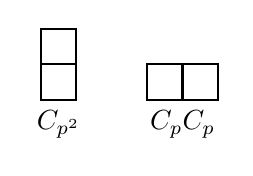
\begin{tikzpicture}[scale=0.45]
            \foreach \x/\h in {0/2} {
                \foreach \y in {1,...,\h} {
                    \draw[thick] (\x,\y-1) rectangle (\x+1,\y);
                }
            }
            \node at (0.5,-0.7) {\(C_{p^2}\)};

            \begin{scope}[xshift=3cm]
                \foreach \x/\h in {0/1,1/1} {
                    \foreach \y in {1,...,\h} {
                        \draw[thick] (\x,\y-1) rectangle (\x+1,\y);
                    }
                }
                \node at (1,-0.7) {\(C_p\cartesianprod C_p\)};
            \end{scope}
        \end{tikzpicture}
    \]
\end{snippetexample}

\begin{snippetexample}{finite-abelian-groups-order-one-hundred-element-counts}{Element orders in abelian groups of order 100}
    The numbers of elements of each possible order are as follows:
    \[
        \begin{array}{c|ccccccccc}
            G\backslash d & 1 & 2 & 4 & 5 & 10 & 20 & 25 & 50 & 100\\
            \hline
            C_{100}
              & 1 & 1 & 2 & 4 & 4 & 8 & 20 & 20 & 40\\
            C_5\cartesianprod C_{20}
              & 1 & 1 & 2 & 24 & 24 & 48 & 0 & 0 & 0\\
            C_2\cartesianprod C_{50}
              & 1 & 3 & 0 & 4 & 12 & 0 & 20 & 60 & 0\\
            C_{10}\cartesianprod C_{10}
              & 1 & 3 & 0 & 24 & 72 & 0 & 0 & 0 & 0
        \end{array}
    \]
    In the cyclic case the entry for \(d\divides100\) is
    \(\eulertotient(d)\). In a direct product, count the tuples whose
    component orders have least common multiple \(d\).
\end{snippetexample}

\begin{snippet}{finite-abelian-direct-product-element-order-counting-method}
    For example, in \(C_5\cartesianprod C_{20}\), the possible component
    orders are
    \[
        d_1\in\{1,5\},
        \qquad
        d_2\in\{1,2,4,5,10,20\}.
    \]
    The number of elements of order \(d\) is
    \[
        \sum_{\lcm(d_1,d_2)=d}
        \eulertotient(d_1)\eulertotient(d_2).
    \]
    The same method applies to every finite direct product of cyclic
    groups.
\end{snippet}

\end{document}
